\section{Reinforcement Learning}

\textbf{Definition:} Reinforcement learning (RL) is a type of machine learning where an agent learns to make decisions by interacting with an environment. The agent receives rewards or punishments based on the actions it takes, and learns to maximize cumulative rewards over time.

\textbf{Basic Loop:}
\begin{itemize}
    \item Agent observes the current \textbf{state} of the environment.
    \item Agent chooses an \textbf{action}.
    \item Environment returns a new \textbf{state} and a \textbf{reward}.
    \item The agent updates its policy based on the experience.
\end{itemize}

\begin{center}
\begin{tikzpicture}[node distance=1.5cm, auto, thick, >=latex]
  \node (agent) [draw, rectangle] {Agent};
  \node (env) [draw, rectangle, right=4cm of agent] {Environment};
  \draw[->] (agent) -- node[above]{Action} (env);
  \draw[->] (env) to[bend right=20] node[below]{New State, Reward} (agent);
\end{tikzpicture}
\end{center}

\subsection*{RLHF: Reinforcement Learning from Human Feedback}

Used for training large language models. The steps:

\begin{enumerate}
    \item Prompt is given to the model.
    \item Model generates multiple responses.
    \item Human annotators rank the responses.
    \item A reward model is trained to predict human preferences.
    \item The main model is updated using reinforcement learning to improve future responses.
\end{enumerate}

\section{Unsupervised Learning}

\textbf{Definition:} Learning patterns in data without labeled outcomes.

\subsection*{Clustering}

Grouping objects such that similar ones are in the same cluster.

\textbf{Applications:}
\begin{itemize}
    \item Genetic research
    \item Image segmentation
    \item Market research
    \item Medical imaging
    \item Social network analysis
\end{itemize}

\subsection*{K-Means Clustering}

\begin{enumerate}
    \item Initialize $k$ cluster centers randomly.
    \item Assign each point to the nearest cluster center.
    \item Recalculate the cluster centers.
    \item Repeat until convergence.
\end{enumerate}

\begin{center}
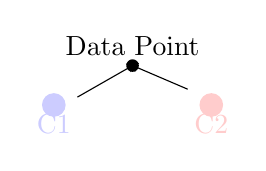
\begin{tikzpicture}
  \fill[blue!20] (0,0) circle (0.15) node[below] {C1};
  \fill[red!20] (2,0) circle (0.15) node[below] {C2};
  \draw[->] (0.3,0.1) -- (1,0.5);
  \draw[->] (1.7,0.2) -- (1,0.5);
  \fill (1,0.5) circle (0.08) node[above] {Data Point};
\end{tikzpicture}
\end{center}

\section{Neural Networks}

\subsection*{Biological Neurons}

Neurons receive electrical impulses from others, process them, and may activate (fire). Artificial Neural Networks (ANNs) are inspired by this concept.

\subsection*{Artificial Neural Network (ANN)}

A neural network is a parameterized function that maps input features $x_1, \ldots, x_n$ to an output $y$:

\[
y = F(x_1, \ldots, x_n)
\]

\textbf{Key Properties:}
\begin{itemize}
    \item \textbf{Input layer:} Accepts features.
    \item \textbf{Hidden layers:} Process and transform input.
    \item \textbf{Output layer:} Produces prediction.
\end{itemize}

\begin{center}
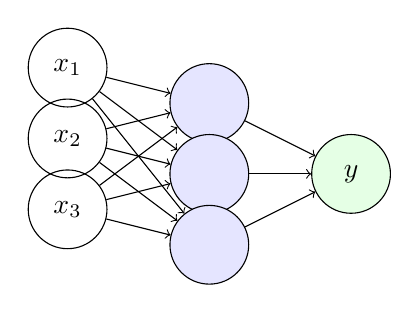
\begin{tikzpicture}[scale=0.9]
  \foreach \i in {1,2,3}
    \node[circle,draw,minimum size=1cm] (I\i) at (0,-\i) {$x_\i$};
  \foreach \i in {1,2,3}
    \node[circle,draw,minimum size=1cm,fill=blue!10] (H\i) at (2,-\i-0.5) {};
  \node[circle,draw,minimum size=1cm,fill=green!10] (O) at (4,-2.5) {$y$};
  
  \foreach \i in {1,2,3}
    \foreach \j in {1,2,3}
      \draw[->] (I\i) -- (H\j);
  \foreach \i in {1,2,3}
    \draw[->] (H\i) -- (O);
\end{tikzpicture}
\end{center}

\textbf{Activation Function: ReLU}

\[
\text{ReLU}(x) = \max(0, x)
\]

\section{Training Neural Networks}

\subsection*{Gradient Descent}

An optimization algorithm used to minimize the loss function by updating weights in the opposite direction of the gradient.

\begin{itemize}
    \item Initialize weights randomly.
    \item Compute gradient of loss with respect to weights.
    \item Update weights:
    \[
    w := w - \eta \cdot \nabla L(w)
    \]
    where $\eta$ is the learning rate.
\end{itemize}

\subsection*{Mini-batch Gradient Descent}

Instead of using the entire dataset, a small random batch is used to compute the gradient.

\subsection*{Backpropagation}

Used to train networks with hidden layers.

\begin{enumerate}
    \item Forward pass to compute output.
    \item Compute loss (error).
    \item Backward pass to propagate error and compute gradients.
    \item Update weights using gradient descent.
\end{enumerate}

\section{Dense Neural Networks}

\begin{itemize}
    \item Each neuron is connected to every neuron in the previous and next layer.
    \item Can learn linear patterns.
    \item Limit: Only learns linearly separable functions.
\end{itemize}

\textbf{Solution:} Use multiple layers (Multilayer Perceptrons) to learn complex patterns.

\textbf{Depth:} Number of layers.\\
\textbf{Width:} Number of neurons per layer.\\
\textbf{Size:} Maximum width of all layers.

\section{Training Strategies}

\subsection*{Train/Validation Split}

\begin{itemize}
    \item 80\% for training
    \item 20\% for validation
\end{itemize}

\textbf{Overfitting:} Model memorizes training data and fails to generalize.\\
\textbf{Underfitting:} Model is too simple or lacks data.

\textbf{Solution:}
\begin{itemize}
    \item Get more data or augment existing data.
    \item Tune hyperparameters (e.g., number of layers, learning rate).
\end{itemize}

\subsection*{Dropout Regularization}

Dropout randomly disables a fraction of neurons during training to prevent overfitting.

\begin{itemize}
    \item Drop rate = proportion of units set to zero.
    \item During inference, all units are used, but activations are scaled by $\frac{1}{1 - \text{rate}}$.
\end{itemize}

\begin{center}
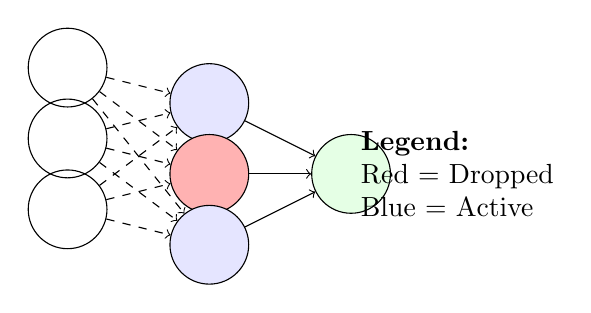
\begin{tikzpicture}[scale=0.9]
  \foreach \i in {1,2,3}
    \node[circle,draw,minimum size=1cm] (I\i) at (0,-\i) {};
  \foreach \i/\c in {1/blue!10,2/red!30,3/blue!10}
    \node[circle,draw,minimum size=1cm,fill=\c] (H\i) at (2,-\i-0.5) {};
  \node[circle,draw,minimum size=1cm,fill=green!10] (O) at (4,-2.5) {};

  \foreach \i in {1,2,3}
    \foreach \j in {1,2,3}
      \draw[->, dashed] (I\i) -- (H\j);
  \foreach \i in {1,2,3}
    \draw[->] (H\i) -- (O);

  \node[align=left] at (5.5, -2.5) {
    \textbf{Legend:} \\
    Red = Dropped \\
    Blue = Active
  };
\end{tikzpicture}
\end{center}